\section[Tool]{Useful tools}

\subsection[Editor]{\cpp editor}

\begin{frame}[fragile]
  \frametitle{\cpp editor}
  \begin{block}{Choose it wisely}
    \begin{itemize}
    \item it can improve dramatically your efficiency by
      \begin{itemize}
      \item coloring the code for you to ``see'' the structure
      \item helping indenting properly
      \item allowing you to navigate easily in the source tree
      \item helping for compilation/debugging
      \end{itemize}
    \end{itemize}
  \end{block}
  \begin{block}{A few tools}
    \begin{description}
    \item[\href{http://www.microsoft.com/}{\beamergotobutton{Visual Studio}}]
      the Microsoft way
    \item[\href{https://www.eclipse.org/}{\beamergotobutton{Eclipse}}]
      similar, but open source and portable
    \item[\href{https://netbeans.org/features/cpp/}{\beamergotobutton{NetBeans}}]
      similar again, also portable
    \item[\href{http://www.gnu.org/software/emacs/}{\beamergotobutton{Emacs}}]
      the expert way. Extremely powerful. Programmable \\
      It is to IDEs what latex is to PowerPoint
    \end{description}
    Choosing one is mostly a matter of taste
  \end{block}
\end{frame}

\subsection[VCS]{Code management}

\begin{frame}[fragile]
  \frametitle{Code management tool}
  \begin{alertblock}{Please use one !}
    \begin{itemize}
    \item even locally
    \item even on a single file
    \item even if you are the only commiter
    \end{itemize}
    It will soon save your day
  \end{alertblock}
  \begin{block}{A few tools}
    \begin{description}
    \item[\href{http://git-scm.com/}{\beamergotobutton{git}}]
      THE best choice. Fast, light, easy to use
    \item[\href{http://mercurial.selenic.com/}{\beamergotobutton{mercurial}}]
      the main alternative
    \item[\href{http://bazaar.canonical.com/en/}{\beamergotobutton{Bazzar}}]
      another alternative
    \item[svn]
      historical, not distributed - DO NOT USE
    \item[CVS]
      archeological, not distributed - DO NOT USE
    \end{description}
  \end{block}
\end{frame}

\begin{frame}[fragile]
  \frametitle{GIT crash course}
  \begin{minted}[gobble=4]{text}
    # mkdir myProject; cd myProject; git init
    Initialized empty Git repository in /tmp/myProject/.git/

    # vim file.cpp; vim file2.cpp
    # git add file.cpp file2.cpp
    # git commit -m "commiting first 2 files"
    [master (root-commit) c481716] commiting first 2 files
    ...

    # git log --oneline
    d725f2e Better STL test
    f24a6ce Reworked examples + added stl one
    bb54d15 implemented template part
    ...

    # git diff f24a6ce bb54d15
  \end{minted}
\end{frame}

\subsection[gcc]{The Compiling Chain}

\begin{frame}[fragile]
  \frametitle{The compiling chain}
  \center
  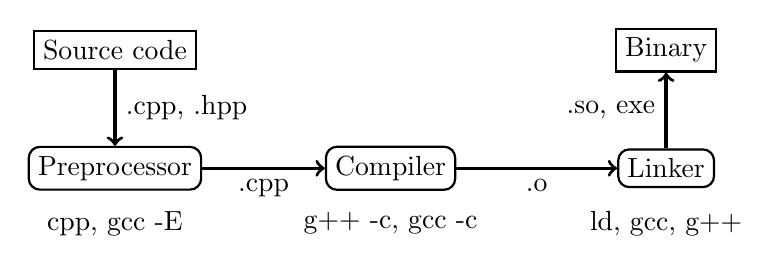
\begin{tikzpicture}
    \draw[thick] node (code) at(0,0) [rectangle,draw] {Source code}
                 node (cpp) at(0, -1.5cm) [rectangle,rounded corners,draw] {Preprocessor}
                 node (gcc) at(3.5cm,-1.5cm) [rectangle,rounded corners,draw] {Compiler}
                 node (ld) at(7cm,-1.5cm) [rectangle,rounded corners,draw] {Linker}
                 node (bin) at(7cm,0) [rectangle,draw] {Binary}
                 node at(0, -2.2cm) {cpp, gcc -E}
                 node at(3.5cm, -2.2cm) {g++ -c, gcc -c}
                 node at(7cm, -2.2cm) {ld, gcc, g++};
    \draw[very thick,->] (code) -- (cpp) node [midway,right] {.cpp, .hpp};
    \draw[very thick,->] (cpp) -- (gcc) node [midway,below] {.cpp};
    \draw[very thick,->] (gcc) -- (ld) node [midway,below] {.o};
    \draw[very thick,->] (ld) -- (bin) node [midway,left] {.so, exe};
  \end{tikzpicture}
  \begin{block}{The steps}
    \begin{description}
    \item[cpp]
        the preprocessor \\
        handles the \# directives (macros, includes) \\
        creates ``complete'' source code
    \item[g++]
        the compiler \\
        creates assembly code from \cpp code
    \item[ld]
        the linker \\
        links several binary files into libraries and executables
    \end{description}
  \end{block}
\end{frame}

\begin{frame}[fragile]
  \frametitle{Compilers}
  \begin{block}{Available tools}
    \begin{description}
    \item[\href{http://gcc.gnu.org/}{\beamergotobutton{gcc}}]
        the most common and most used\\
        free and open source
    \item[\href{http://clang.llvm.org/}{\beamergotobutton{clang}}]
        drop-in replacement of gcc \\
        slightly better error reporting \\
        free and open source
    \item[\href{http://software.intel.com/en-us/intel-compilers}{\beamergotobutton{icc}}]
        the intel compiler \\
        proprietary \\
        optimized for Intel hardware
    \item[\href{http://www.microsoft.com/}{\beamergotobutton{Visual \cpp}}]
      the Windows way
    \end{description}
  \end{block}
  \begin{alertblock}{My prefered choice today}
    \begin{itemize}
      \item \alert{gcc} as the de facto standard in HEP
      \item \hspace{0pt}\alert{clang} in parallel to catch more bugs
    \end{itemize}
  \end{alertblock}
\end{frame}

\begin{frame}[fragile]
  \frametitle{Useful compiler options (gcc/clang)}
  \begin{block}{Get more warnings}
    \begin{description}
      \item[-Wall -Wextra] the way to get all warnings
      \item[-Werror] the way to force yourself to look at warnings
    \end{description}
  \end{block}
  \begin{block}{Around optimization}
    \begin{description}
      \item[-g] add debug symbols
      \item[-O0, -O2] 0 = no optimization, -O2 = optimized
    \end{description}
  \end{block}
  \begin{block}{Compilation environment}
    \begin{description}
      \item[\texttt{-I} \textless{}path\textgreater] where to find header files
      \item[\texttt{-L} \textless{}path\textgreater] where to find libraries
      \item[\texttt{-l} \textless{}name\textgreater] link with libname.so
      \item[\texttt{-E / -c}] stop after preprocessing / compilation
    \end{description}
  \end{block}
\end{frame}

\begin{frame}[fragile]
  \frametitle{Makefiles}
  \begin{block}{Why to use them}
    \begin{itemize}
    \item an organized way of describing building steps
    \item avoids a lot of typing
    \end{itemize}
  \end{block}
  \begin{block}{Several implementations}
    \begin{itemize}
    \item raw Makefiles : suitable for small projects
    \item cmake : portable, the current best choice
    \item automake : portable but complex
      \end{itemize}
  \end{block}
  \begin{minted}{makefile}
    test : test.cpp libpoly.so
        $(CXX) -Wall -Wextra -o $@ $^
    libpoly.so: Polygons.cpp
        $(CXX) -Wall -Wextra -shared -fPIC -o $@ $^
    clean:
        rm -f *o *so *~ test test.sol
  \end{minted}
\end{frame}

\begin{frame}[fragile]
  \frametitle{Compiler chain}
  \begin{alertblock}{Exercise Time}
    \begin{itemize}
    \item go to code/polymorphism
    \item preprocess Polygons.cpp (cpp or gcc -E -o output)
    \item compile Polygons.o and test.o (g++ -c -o output)
    \item use nm to check symbols
    \item see link statement using g++ -v
    \item see library dependencies with ldd
    \item look at the Makefile
    \item try make clean; make
    \end{itemize}
  \end{alertblock}
\end{frame}

\subsection[gdb]{Debugging}

\begin{frame}[fragile]
  \frametitle{Debugging}
  \begin{alertblock}{The problem}
    \begin{itemize}
      \item everything compiles fine (no warning)
      \item but crashes at run time
      \item no error message, no clue
    \end{itemize}
  \end{alertblock}
  \pause
  \begin{block}{The solution : debuggers}
    \begin{itemize}
    \item dedicated program able to stop execution at any time
    \item and show you where you are and what you have
    \end{itemize}
  \end{block}
  \pause
  \begin{block}{Existing tools}
    \begin{description}
    \item[\href{http://www.sourceware.org/gdb/}{\beamergotobutton{gdb}}]
      THE main player
    \item[\href{http://lldb.llvm.org/}{\beamergotobutton{lldb}}]
      the debugger coming with clang, still young
    \item[\href{http://software.intel.com/en-us/articles/idb-linux}{\beamergotobutton{idb}}]
      the intel debugger, proprietary
    \end{description}
  \end{block}
\end{frame}

\begin{frame}[fragile]
  \frametitle{gdb crash course}
  \begin{block}{start gdb}
    \begin{itemize}
    \item gdb \textless{}program\textgreater
    \item gdb \textless{}program\textgreater \textless{}core file\textgreater
    \end{itemize}
  \end{block}
  \begin{block}{inspect state}
    \begin{description}
    \item[bt] prints a backtrace
    \item[print \textless{}var\textgreater] prints current content of the variable
    \item[list] show code around current point
    \item[up/down] go up or down in call stack
    \end{description}
  \end{block}
  \begin{block}{breakpoints}
    \begin{description}
    \item[break \textless{}function\textgreater] puts a breakpoint on function entry
    \item[break \textless{}file\textgreater:\textless{}line\textgreater] puts a breakpoint on that line
    \end{description}
  \end{block}
\end{frame}

\begin{frame}[fragile]
  \frametitle{gdb}
  \begin{alertblock}{Exercise Time}
    \begin{itemize}
    \item go to code/debug
    \item compile, run, see the crash
    \item run it in gdb
    \item inspect backtrace, variables
    \item find problem and fix bug
    \item try stepping, breakpoints
    \item use -Wall -Wextra and see warning
    \end{itemize}
  \end{alertblock}
\end{frame}

\subsection[valgrind]{The Valgrind family}

\begin{frame}[fragile]
  \frametitle{The valgrind family}
  \begin{block}{Valgrind fundamentals}
    \begin{itemize}
    \item valgrind is a framework for different tools
    \item a processor simulator allowing checks in between instructions
    \item slow (10-50 times slower than normal execution)
    \item easy to use : ``valgrind \textless{}your executable\textgreater''
      \begin{itemize}
      \item no recompilation
      \item better with -g -O0, but not strictly needed
      \end{itemize}
    \item it is free and open source
    \end{itemize}
  \end{block}
  \pause
  \begin{block}{Main tools}
    \begin{description}
      \item[memcheck] a memory checker (default tool) and leak detector
      \item[callgrind] a call graph builder
      \item[helgrind] a race condition detector
    \end{description}
  \end{block}
\end{frame}

\begin{frame}[fragile]
  \frametitle{memcheck}
  \begin{block}{}
    \begin{itemize}
      \item keeps track of all memory allocations and deallocations
      \item is able to detect accesses to non allocated memory
      \item and even tell you when it was deallocated if it was
      \item or what it the closest array in case of overflow
      \item is able to list still allocated memory when program exits\\
        (memory leaks detection)
    \end{itemize}
  \end{block}
\end{frame}

\begin{frame}[fragile]
  \frametitle{valgrind}
  \begin{alertblock}{Exercise Time}
    \begin{itemize}
    \item go to code/valgrind
    \item compile, run, it should work
    \item run with valgrind, see the problem
    \item fix the problem
      \vspace{.3cm}
    \item go back to the code/debug exercise
    \item check it with valgrind
    \item analyze the issue, see that the variance was biaised
    \item fix the issue
    \end{itemize}
  \end{alertblock}
\end{frame}

\begin{frame}[fragile]
  \frametitle{memcheck}
  \begin{alertblock}{Exercise Time}
    \begin{itemize}
    \item go to code/memcheck
    \item compile, run, it should work
    \item run with valgrind, see LEAK summary
    \item run with -{}-leak-check=full to get details
    \item analyze and correct it
    \end{itemize}
  \end{alertblock}
\end{frame}

\begin{frame}[fragile]
  \frametitle{callgrind and kcachegrind}
  \begin{block}{callgrind}
    \begin{itemize}
      \item keeps track of all function calls
      \item and time spent in each function
      \item build statistics on calls, CPU usages and more
      \item outputs flat statistics file, quite unreadable
    \end{itemize}
  \end{block}
  \begin{block}{kcachegrind}
    \begin{itemize}
      \item a gui exploiting statistics built by callgrind
      \item able to browse graphically the program calls
      \item able to ``graph'' CPU usage on the program structure
    \end{itemize}
  \end{block}
\end{frame}

\begin{frame}[fragile]
  \frametitle{callgrind}
  \begin{alertblock}{Exercise Time}
    \begin{itemize}
    \item go to code/callgrind
    \item compile, run, it will be slow
    \item change nb iterations to 20
    \item run with valgrind -{}-tool=callgrind
    \item look at output with kcachegrind
    \item change fibo call to fibo2
    \item observe the change in kcachegrind
    \end{itemize}
  \end{alertblock}
\end{frame}

\begin{frame}[fragile]
  \frametitle{helgrind}
  \begin{block}{}
    \begin{itemize}
      \item keeps track of all pthreads activity
      \item in particular keeps track of all mutexes
      \item builds a graph of dependencies of the different actions
      \item works on the resulting graph to detect:
        \begin{itemize}
        \item possible dead locks
        \item possible data races
        \end{itemize}
    \end{itemize}
  \end{block}
  \pause
  \begin{alertblock}{}
    Note the ``possible''. It finds future problems !
  \end{alertblock}
\end{frame}

\begin{frame}[fragile]
  \frametitle{helgrind}
  \begin{alertblock}{Exercise Time}
    \begin{itemize}
    \item go to code/helgrind
    \item compile, run
    \item check it with valgrind. See strange behavior \\
      but no explanation
    \item check it with valgrind -{}-tool=helgrind
    \item understand issue and fix
    \end{itemize}
  \end{alertblock}
\end{frame}

\subsection[static]{Static code analysis}

\begin{frame}[fragile]
  \frametitle{Static analysis}
  \begin{alertblock}{The problem}
    \begin{itemize}
    \item all the tools discussed so far work on binaries
    \item they analyze the code being run
    \item so there is a coverage problem (e.g. for error cases)
    \end{itemize}
  \end{alertblock}
  \pause
  \begin{block}{A (partial) solution : analyzing the source code}
    \begin{itemize}
    \item build a graph of dependencies of the calls
    \item use graph tools to detect potential memory corruptions,
      memory leaks ot missing initializations
    \end{itemize}
  \end{block}
  \pause
  \begin{block}{Existing tools}
    \begin{description}
    \item[\href{http://www.coverity.com/}{\beamergotobutton{Coverity}}]
      proprietary tool, the most complete
    \item[\href{http://cppcheck.sourceforge.net/}{\beamergotobutton{cppcheck}}]
      free and opensource, but less complete
    \item[\href{http://clang-analyzer.llvm.org/}{\beamergotobutton{scan-build}}]
      the clang source analyzer
    \end{description}
  \end{block}
\end{frame}

\begin{frame}[fragile]
  \frametitle{cppcheck}
  \begin{alertblock}{Exercise Time}
    \begin{itemize}
    \item go to code/cppcheck
    \item compile, run, see that it works
    \item use valgrind : no issue
    \item use cppcheck, see the problem
    \item analyze the issue, and fix it
    \item bonus : understand why valgrind did not complain \\
      and how the standard deviation could be biased \\
      hint : use gdb and check addresses of v and diffs
    \end{itemize}
  \end{alertblock}
\end{frame}
